\documentclass{article}
\usepackage[utf8]{inputenc}
\usepackage[T1]{fontenc}
\usepackage[utf8]{inputenc}
\usepackage{lmodern}
\usepackage[a4paper, margin=1in]{geometry}
\usepackage{graphicx}
\graphicspath{ {./images/} }

\usepackage{minted}
\large
\title{CSE 344 HW4}
\begin{document}
\begin{titlepage}
	\begin{center}
    \line(1,0){300}\\
    [0.65cm]
	\huge{\bfseries CSE344 HW4}\\
	\line(1,0){300}\\
	\textsc{\Large Initiation to POSIX threads}\\
	\textsc{\LARGE Homework Business}\\
	[5.5cm]     
	\end{center}
	\begin{flushright}
		\textsc{\Large Hüsnü AKÇAK\\161044112}\\
		[0.5cm]
	
	\end{flushright}
\end{titlepage}

\section*{Program Setup}

\subsection*{General Design}
   First the semaphores are initialized.
   Then the two text files are read. Worker struct array is initialized according to the student file, the homework queue is initialized according to homework file.
   
   The first thread which I started is hwOwner, it starts its execution, read the hw file, fill the homework queue, then let the main thread know it has finished its reading and filled the queue, afterwards main thread run all the worker threads and orchestrate them to consume the homework queue.
   
   The program could be terminated in three ways, 1-homeworks done, 2-out of money, 3-keyboard interrupt. For all three scenario main thread perform pthread join for worker threads, thread H detached itself, all the dynamic allocated resources are freed, the files are closed, the semaphores are destroyed then main thread exit.

   Max name length for worker threads is 255.
   
   Max speed for worker threads is 6.

\subsection*{Orchestration of Worker Threads}
    It is managed from organizeThreads function, this function is executed by main thread. 
    
    A loop continues as long as there is a hw in the queue and there is enough money to effort homework delegation. Also if a keyboard interrupt(CTRL-C) is received, the execution is nicely terminated.
    
    At every step in the loop;
        It is controlled if there is an available and affordable worker thread, if so the most convenient one is selected and the current homework is delegated. 

    The most convenient thread is selected according to priority type of the homework, it could be
    C, S, Q as indicated in the instruction document of this assignment. There are three function exist for each different type of selection as;
    
    int getMostQualifiedIndex();
    int getFasterIndex();
    int getCheapestIndex();
    
    They return the index of most suitable worker thread.

\subsection*{Worker threads}
    The function is worker.
    
    As soon as they start, they wait for the main thread to call them for homework delegation, or termination indication.
    
    When they awake by the main thread, it is controlled if there is a job, or should that thread need to be terminate, or if there is not enough money for its price it also means termination.
    
    If all is good and the worker thread start do to given homework, it decreases the available money, increases the studied homework by her, go to sleep for a certain amount of seconds, then be ready to receive a new instruction from the main thread.
    
    
\subsection*{Homework owner thread }
    This thread is responsible to read all her homeworks from the file, fill the hwQueue, notify main thread that the queue is ready. And wait for the termination instruction from main thread. 
    
    The termination message could be 3 different type, homeworks are done, we are out of money, or a keyboard interruption(CTRL-C). In all three cases the thread detached herself.
    
\section*{Screen Shots}
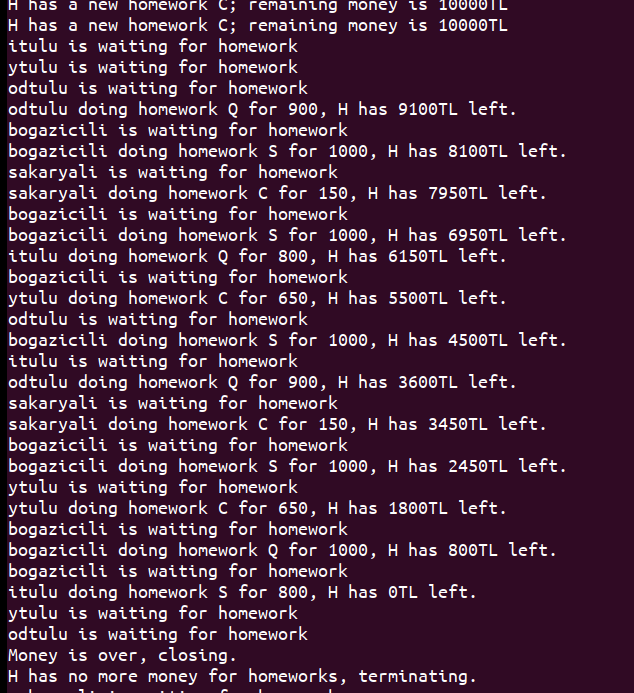
\includegraphics[]{1.png}


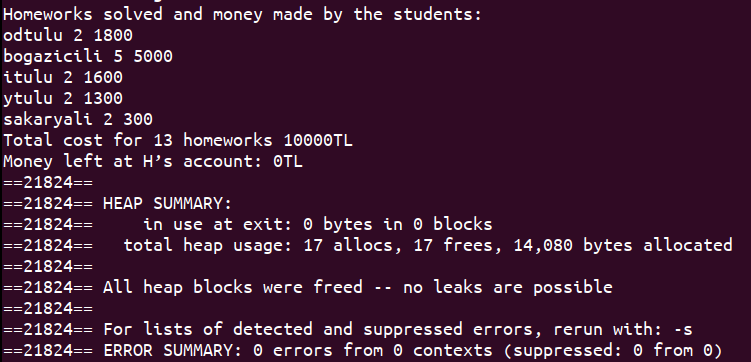
\includegraphics[]{2.png}


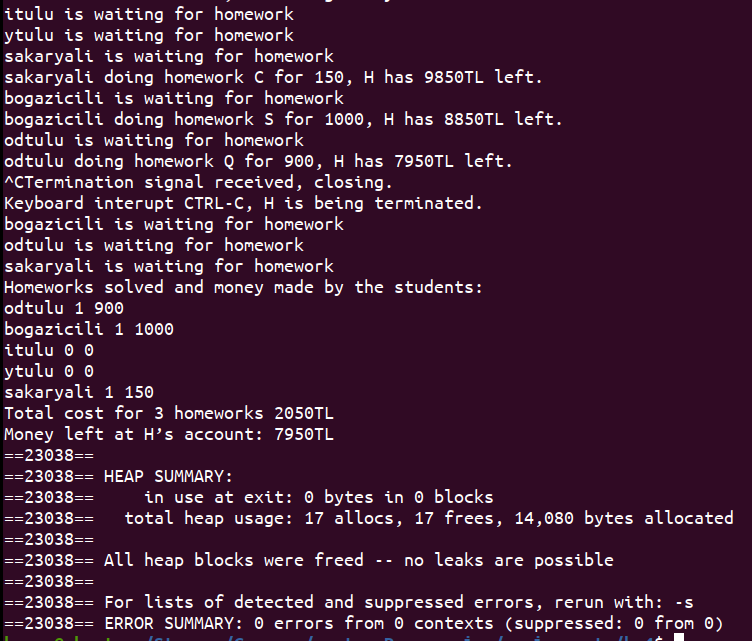
\includegraphics[]{3.png}



\end{document}











